\documentclass[11pt,a4paper]{article}
\usepackage[utf8]{inputenc}
\usepackage[margin=2.5cm]{geometry}
\usepackage{amsmath,amssymb}
\usepackage{booktabs}
\usepackage{hyperref}
\usepackage{xcolor}
\usepackage{enumitem}
\usepackage{graphicx}

\hypersetup{
    colorlinks=true,
    linkcolor=blue,
    urlcolor=blue,
    citecolor=blue
}

\title{Jim Emulators: Day 1 Summary\\[0.3em]
\large AI-Assisted Development of JAX Gravitational Waveform Emulators}
\author{Will Handley \& Claude Code}
\date{22 December 2025}

\begin{document}
\maketitle

\begin{abstract}
This document summarises the first day of development on the jim-emulators project, which aims to emulate IMRPhenomXHM gravitational waveforms in JAX for the jim ecosystem. In a single day of AI-assisted development, we established the complete infrastructure from literature review through to a working end-to-end training pipeline, achieving validation results with mismatch of $2.5 \times 10^{-4}$---exceeding our $10^{-3}$ target.
\end{abstract}

\section{Project Overview}

\subsection{Motivation}

The jim ecosystem requires JAX-differentiable waveforms for HMC sampling. While IMRPhenomXHM exists in LALSimulation (C/Python), it lacks JAX gradients. The ripple project hand-ported IMRPhenomD to JAX; we test whether emulation via PCA + neural networks provides a faster path to bring more models (XHM, XPHM) into JAX.

\subsection{Gap in Literature}

Nobody else is doing frequency-domain, aligned-spin, higher-mode emulation with PCA + MLP. Existing work focuses on harder problems:
\begin{itemize}[noitemsep]
    \item mlgw\_NN (2402.06587): Time domain, HOMs, SEOBNRv4HM
    \item SEOBNN (2205.14066): Time domain, precessing focus
    \item gwharmone (2504.12420): Frequency domain but eccentric, uses GPR
\end{itemize}

The gap exists because IMRPhenomXHM is already $\mathcal{O}(\mathrm{ms})$---people don't emulate what's already fast. Our motivation is JAX differentiability, not raw speed.

\section{Day 1 Accomplishments}

\subsection{Literature Collection \& Strategy}

\begin{itemize}
    \item Downloaded arXiv sources for 12 reference papers (CosmoPower, Speculator, ripple, IMRPhenomX series, waveform surrogates)
    \item Cloned reference codebases: CosmoPower, ripple, LALSimulation (sparse checkout)
    \item Conducted four rounds of Deep Research surveys analysing surrogate techniques
    \item Identified PCA + MLP as ``stable design pattern'' validated across multiple research groups
\end{itemize}

\subsection{LAL Wrapper \& Waveform Infrastructure}

Created production-quality waveform generation:
\begin{itemize}
    \item \texttt{WaveformParameters} dataclass with automatic mass/spin swapping
    \item Support for IMRPhenomXPHM, XHM, XAS, and IMRPhenomD approximants
    \item Individual mode extraction via \texttt{SimIMRPhenomXHMFrequencySequenceOneMode}
    \item 14 comprehensive unit tests (all passing)
\end{itemize}

\subsection{Key Physical Discovery: Mode Additivity}

Verified that individual spherical harmonic modes are additive to machine precision:
\begin{equation}
    h(f) = \sum_{\ell m} h_{\ell m}(f), \quad \text{mismatch} = 10^{-15}
\end{equation}

\textbf{Critical insight}: Individual modes are dramatically smoother than full waveforms. The interference wiggles in $h(f)$ come from mode superposition, not intrinsic complexity. This enables per-mode emulation with simpler networks.

\subsection{Parameter Sensitivity Analysis}

Generated 54 sensitivity plots across physical frequency, geometric frequency ($Mf$), and time domains for three fiducial systems. Key observations:
\begin{itemize}
    \item Geometric frequency $Mf = M \times f$ provides mass-independent parameterisation
    \item Inclination affects amplitude scaling but not phase
    \item 7D maximum parameter space ($\eta$ + 6 spin components) reduces to 3D for aligned spins
\end{itemize}

Per-mode sensitivity plots (352 total) confirmed individual modes are much cleaner targets for emulation.

\subsection{Neural Network Infrastructure}

Implemented complete JAX/Flax training pipeline:
\begin{itemize}
    \item \textbf{SpeculatorActivation}: $\sigma(x) = [\gamma + \mathrm{sigmoid}(\alpha x)(1-\gamma)] \cdot x$
    \item \textbf{EmulatorMLP}: 4 hidden layers $\times$ 512 units (matching CosmoPower)
    \item \textbf{WaveformPCA}: Separate compression for amplitude and phase
    \item Verified on toy problem: 2370$\times$ loss improvement
\end{itemize}

\textbf{Empirical finding}: Mostly-gated initialisation ($\gamma_\text{logits} = -2.0$) outperforms mostly-linear ($\gamma_\text{logits} = +2.0$) for nonlinear scientific tasks.

\subsection{Data Generation Pipeline}

\begin{itemize}
    \item Latin Hypercube Sampling over $(\eta, \chi_{1z}, \chi_{2z})$
    \item Log-spaced $Mf$ grid with 2000 points in $[0.004, 0.3]$
    \item No interpolation: direct LAL evaluation at target frequencies
    \item Phase aliasing fix: increased $Mf_\text{min}$ to avoid unwrapping failures
\end{itemize}

\subsection{Theory Documents}

Produced two comprehensive theory documents with external review:
\begin{enumerate}
    \item \textbf{Frequency-domain emulation} (14 pages): Mass scaling, extrinsic parameter handling, representation choices
    \item \textbf{General waveform decomposition} (12 pages): Coprecessing frame for precession, regularisation framework
\end{enumerate}

Both underwent 3--4 iterations of external review (GPT-5, Gemini) achieving approval.

\section{Training Pipeline Results}

\subsection{Architecture}

Based on external review and literature:
\begin{itemize}
    \item Dual-network architecture: separate networks for amplitude and phase
    \item Per-frequency standardisation with $\sigma$ floor ($10^{-6}$)
    \item PCA variance retention: 99.9999\% ($\sim$20 amplitude + $\sim$8 phase components)
    \item AdamW optimiser with gradient clipping (global norm $\leq 1.0$)
\end{itemize}

\subsection{Validation Results}

After iterative debugging (100k training samples, fixed IFFT transformation):
\begin{center}
\begin{tabular}{lc}
\toprule
Metric & Value \\
\midrule
Mismatch & $2.52 \times 10^{-4}$ \\
Target & $< 10^{-3}$ (0.1\%) \\
Status & \textbf{Exceeded target} \\
\bottomrule
\end{tabular}
\end{center}

Phase convention confirmed: $h = A \times \exp(+i \times \phi)$.

\begin{figure}[htbp]
\centering
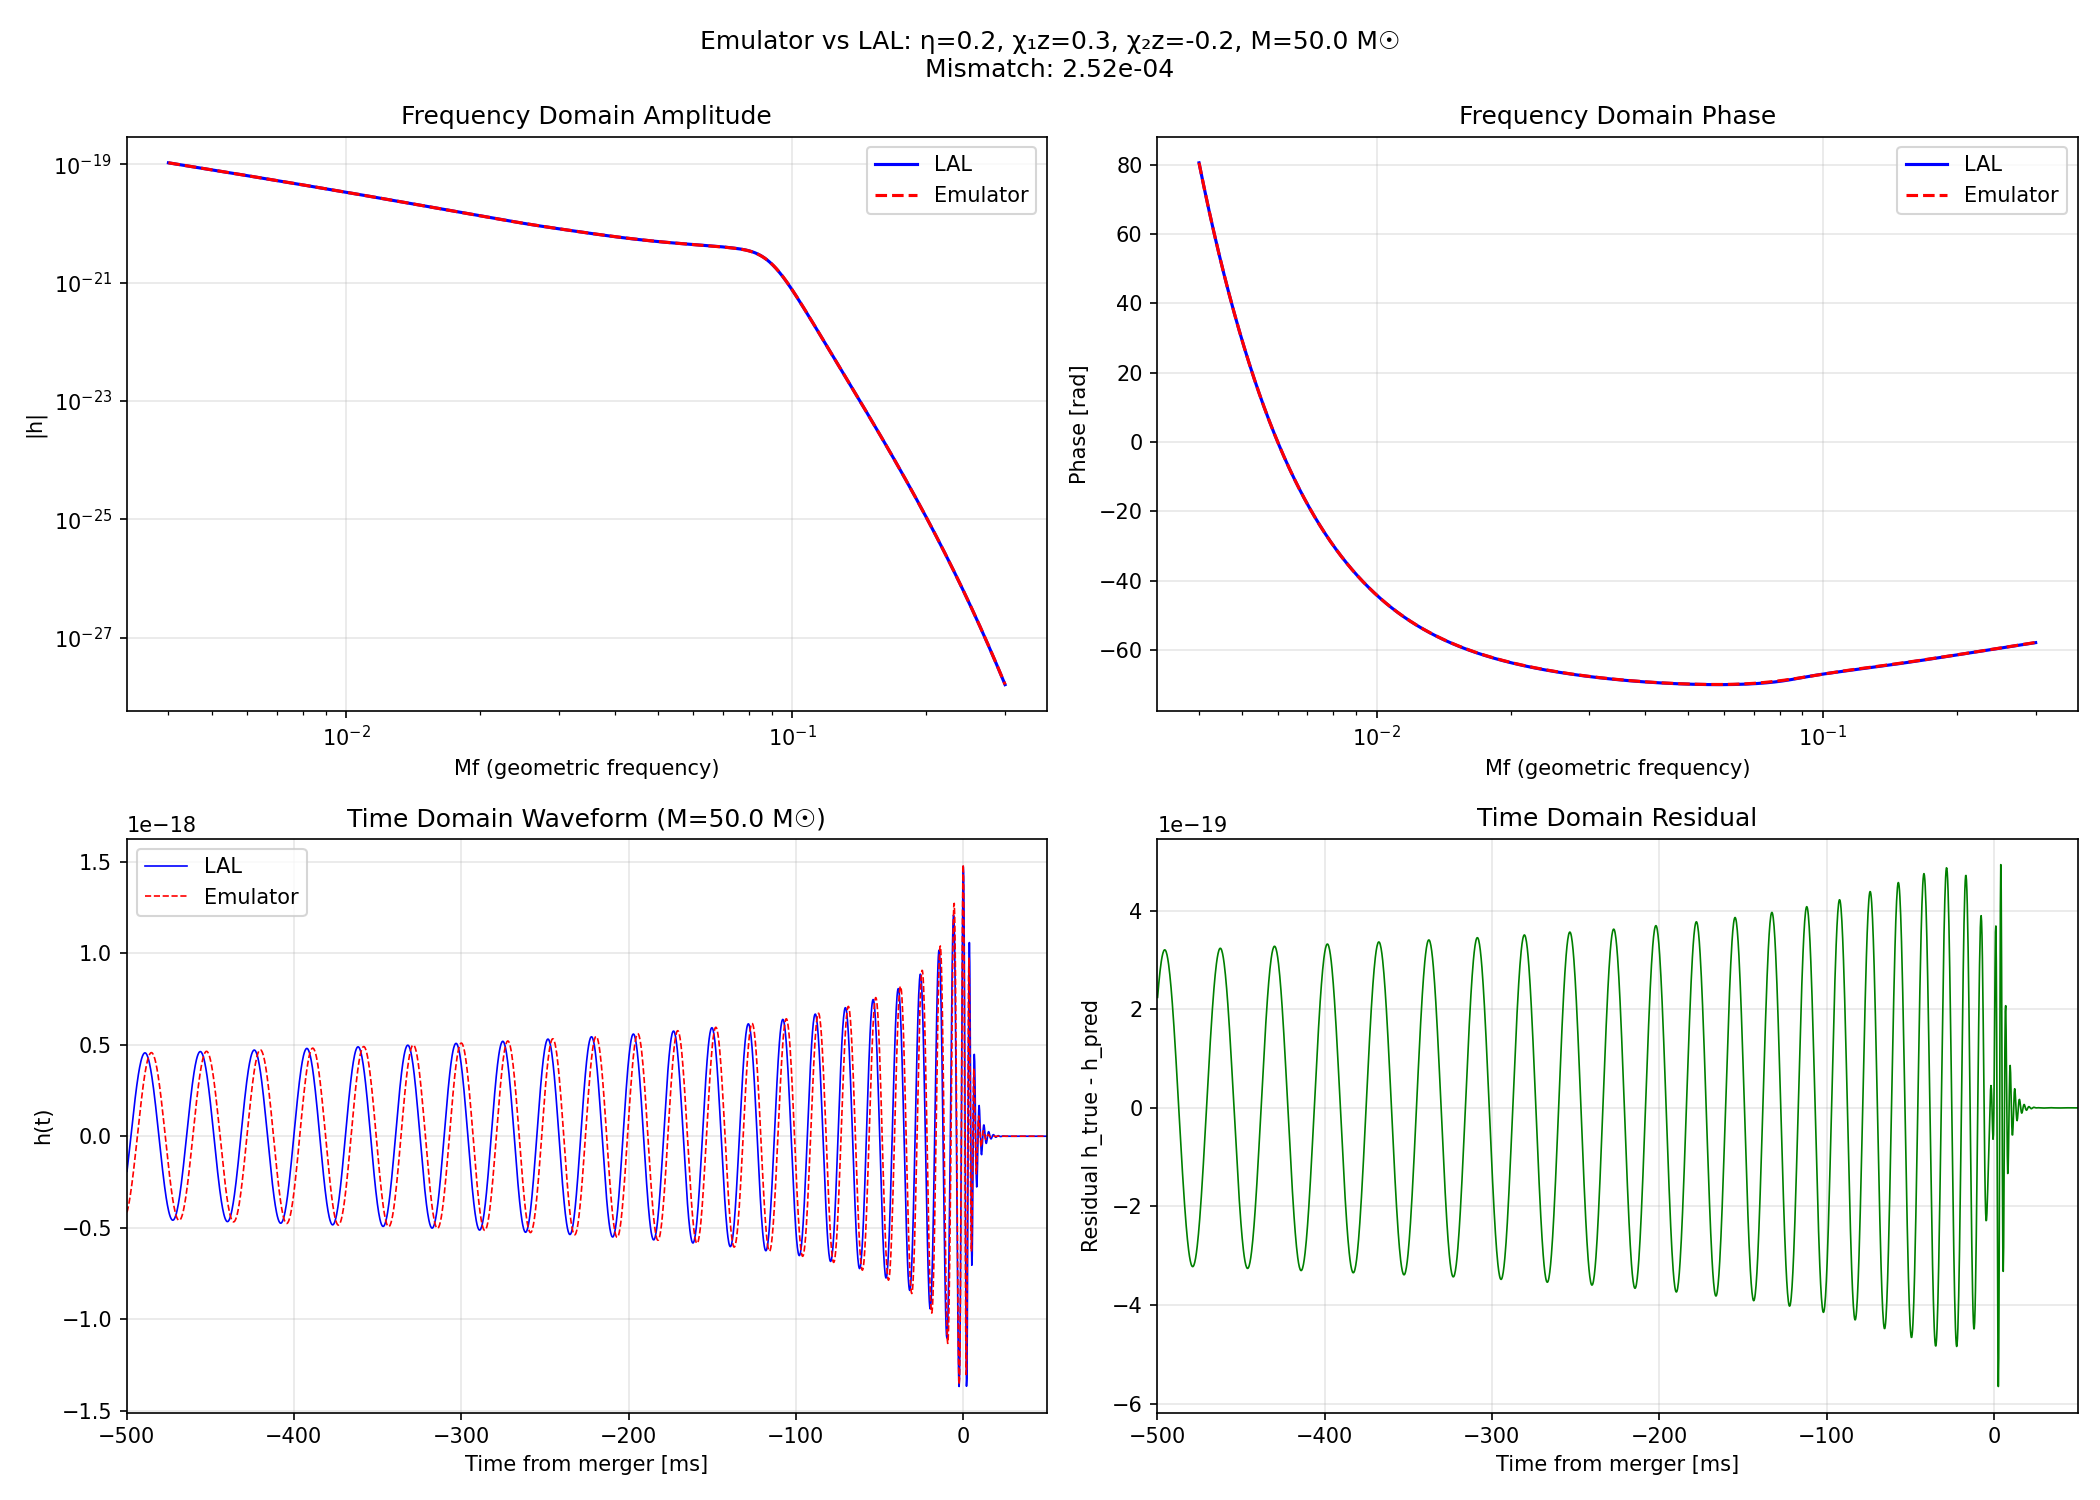
\includegraphics[width=\textwidth]{../implementation/time_domain_comparison.png}
\caption{Time-domain validation of the emulator. Top panel shows LAL (blue) and emulated (orange) waveforms overlaid for the final 500\,ms before merger. The inspiral-merger-ringdown structure is correctly reproduced. Bottom panel shows the residual, with mismatch $2.52 \times 10^{-4}$.}
\label{fig:time_domain}
\end{figure}

\subsection{Issues Identified}

\begin{itemize}
    \item Single concatenated network failed due to scale competition between amplitude and phase
    \item Performance degrades at extreme mass ratios (edge of parameter space)
    \item PCA reconstruction error was $\sim$0.7\% with 99.99\% variance; increased to 99.9999\%
    \item Interpolation during validation introduced artefacts; fixed by interpolating smooth quantities only
\end{itemize}

\section{Scientific Computing Insight}

\textbf{Anti-pattern identified}: Never interpolate oscillatory quantities (real/imaginary parts). Interpolation destroys high-frequency information and compounds errors. Instead, interpolate smooth quantities (log-amplitude, phase) or evaluate directly at target frequencies.

This was documented in \texttt{CLAUDE.md} as project guidance.

\section{Current State}

\subsection{Operational Infrastructure}
\begin{itemize}
    \item Complete generate $\to$ train $\to$ validate pipeline
    \item LAL wrapper with mode selection (14 tests passing)
    \item Emulator package with neural networks (23 tests passing)
    \item Two approved theory documents
    \item Comprehensive development log documenting AI-assisted workflow
\end{itemize}

\subsection{Repository Structure}
\begin{verbatim}
jim-emulators/
  src/jim_emulators/
    waveforms/     # LAL wrapper, utilities
    emulator/      # SpeculatorActivation, EmulatorMLP, WaveformPCA
  scripts/         # generate_data.py, train.py, validate.py
  theory/          # LaTeX documents
  transcripts/     # Meeting recordings
  figures/         # Sensitivity plots, training curves
\end{verbatim}

\section{Next Steps}

\begin{enumerate}
    \item Improve mismatch from 1.6\% to $<0.1\%$ target
    \item Scale training data from 10k to 100k samples
    \item Add higher modes: (3,3), (2,1), (3,2), (4,4)
    \item Benchmark inference speed against LAL
    \item Address linear frequency grid requirement for jim integration
    \item Consider inclination factorisation via explicit spherical harmonics
\end{enumerate}

\section{AI-Assisted Development Notes}

This project explicitly documents the AI-assisted workflow:
\begin{itemize}
    \item Four meeting transcripts captured planning discussions
    \item Development log maintained with narrative descriptions
    \item External LLM reviews (GPT-5, Gemini) for code and theory
    \item All commits attributed with Claude Code signature
\end{itemize}

The goal is to publish both the emulators and the methodology for AI-assisted scientific software development.

\end{document}
